\documentclass{article}

% If you're new to LaTeX, here's some short tutorials:
% https://www.overleaf.com/learn/latex/Learn_LaTeX_in_30_minutes
% https://en.wikibooks.org/wiki/LaTeX/Basics

% Formatting
\usepackage[utf8]{inputenc}
\usepackage[margin=1in]{geometry}
\usepackage[titletoc,title]{appendix}

% Math
% https://www.overleaf.com/learn/latex/Mathematical_expressions
% https://en.wikibooks.org/wiki/LaTeX/Mathematics
\usepackage{amsmath,amsfonts,amssymb,mathtools}

% Images
% https://www.overleaf.com/learn/latex/Inserting_Images
% https://en.wikibooks.org/wiki/LaTeX/Floats,_Figures_and_Captions
\usepackage{graphicx,float}

% Tables
% https://www.overleaf.com/learn/latex/Tables
% https://en.wikibooks.org/wiki/LaTeX/Tables

% Algorithms
% https://www.overleaf.com/learn/latex/algorithms
% https://en.wikibooks.org/wiki/LaTeX/Algorithms
\usepackage[ruled,vlined]{algorithm2e}
\usepackage{algorithmic}

% Code syntax highlighting
% https://www.overleaf.com/learn/latex/Code_Highlighting_with_minted
\usepackage{listings}
%\usepackage{minted}
%\usemintedstyle{borland}

\usepackage{hyperref}
\usepackage{subcaption}
\usepackage{bm}

% References
% https://www.overleaf.com/learn/latex/Bibliography_management_in_LaTeX
% https://en.wikibooks.org/wiki/LaTeX/Bibliography_Management
%\usepackage{biblatex}
%\addbibresource{references.bib}

% Title content
\title{AMATH 582 Homework Two: Shredding Analysis}
\author{Daniel W. Crews}
\date{February 10, 2021}

\begin{document}

\maketitle

% Abstract
\begin{abstract}
  Spectral analysis consists of far more than determination of the Fourier coefficients of a time series. This numerical experiment explores the spatial distribution of a signal's frequency spectrum (or spectrogram) through the pratical examples of classic shredding moments in music history (here, Guns and Roses and Pink Floyd). To compute the spectrograms a short-time (masked) Fourier transform is used, and in particular this report explores its filtering using the Wigner distribution function of the time series. Here the Wigner function is computed as an $\mathcal{O}(N^2)$ operation in terms of the Fourier coefficients.
    %Signal processing is used ubiquitously in science and engineering. This simple numerical experiment explores an important aspect of signal analysis, namely statistical averaging of a spectral time series to eliminate noise and thereby identify center frequencies. Here the time series consists of a spatial wavefield which is denoised via Gaussian filtering about the identified frequency to determine a trajectory. While the technique explored in this report is quite elementary compared to more sophisticated signal processing approaches, it conveys the essential elements of, for example, a radar or sonar tracking system. %In this case such a trajectory is determined from a noisy waveform in a time series of three spatial dimensions. 
\end{abstract}

% Introduction and Overview
\section{Introduction and Overview}
The purpose of this work is to visualize some of the most famous shredding in rock and roll history (Pink Floyd and Guns and Roses (GNR)) by construction of a spectrogram. Section \ref{theory} outlines the theory of the combined Gabor-Wigner distribution used for the spectrogram, followed by a section detailing implementation of the algorithm. Results are presented for the opening guitar riff in GNR, bass line in Floyd, and a stab at the Floyd guitar solo. The attached appendices describing elements of Wigner distributions are hoped not to count towards the overall page limit and included merely for completeness. The report itself is kept concise.

% This report describes an algorithm used to denoise the signal via a statistical method and to identify the submarine's trajectory. It begins with a brief theoretical overview of the methods used, and proceeds to a discussion of the details of the code used to implement the methods. There is then a discussion of results identifying the three-dimensional trajectory, along with a suggested search area for a submarine-tracking aircraft and the likely frequency of the submarine. The report is kept brief without sacrificing clarity.

% Theoretical Background
\section{Theoretical Background}\label{theory}
\subsection{Time-frequency analysis}
The Fourier decomposition of a periodic signal $f(t+L)=f(t)$ exchanges the coordinate $t$ for the distribution $\hat{f}(\omega)$ in frequency $\omega$, which when continuous yet periodic in $t$ is discrete in $\omega$,
\begin{equation}
  f(t) = \sum_{n=-\infty}^\infty c_ne^{i\omega_nt},\quad\quad \hat{f}(\omega) = \sum_{n=-\infty}^\infty c_n\delta(\omega - \omega_n),\quad\quad \omega_n = \frac{2\pi}{L}n.
\end{equation}
Each spectral coefficient is found through integration with the unmasked Fourier integral kernel,
\begin{equation}
  c_n = \frac{1}{L}\int_0^L f(t)e^{-i\omega_nt}dt.
\end{equation}
The total frequency distribution $\hat{f}(\omega)$ counts the orthogonal components of $f(t)$ but is completely delocalized (in coordinate $t$). On the other hand the original distribution $f(t)$ does not convey local frequencies. However, the spatial distribution of signal frequencies is of broad interest in science, demonstrated by the following abstract example. Consider energy distributed across a range of frequencies with mean zero,
\begin{equation}
  \psi(t) = \sum_{n=1}^N\cos(2\pi nt + \varphi(n))
\end{equation}
with $\varphi$ a phase variable. If $\varphi(n)$ is randomly distributed in $[0,2\pi)$ then $\psi$ is white noise, yet if $\varphi \equiv 0$ then the signal energy is increasingly singularly concentrated in coordinate $t$ (i.e. $\lim_{N\to\infty}\psi(t)\to\delta(t)$). Both functions have the same amplitude distribution $|\hat{f}(\omega)|$ (where phase information is discarded).

The goal of time-frequency analysis is to establish a function which can capture the spatial distribution of signal energy and describe its frequency contents as well. The two classic approaches are the short-time method (Gabor transform) and the instantaneous autocorrelation transform (or Wigner function).
\subsection{Masked Fourier transform (Gabor method)}
The short-time Fourier transform, also called the Gabor transform, masks the Fourier kernel with a window,
\begin{equation}
  \mathcal{G}_n(t) = \frac{1}{L}\int_{0}^L f(\tau)g(t,\tau)e^{-i\omega_n\tau}d\tau
\end{equation}
where $g(t,\tau)$ is an integrable window function which should be translationally covariant and even about $t=\tau$ \cite{kutz}. Common choices of window are the Gaussian and the bump function. The bump function is used for this study because it has compact support and can slide across a periodic domain without overlapping itself,
\begin{equation}
  g(t-\tau) = \exp(1)\exp\Big(\frac{-a^2}{a^2-(t-\tau)^2}\Big),\quad t-\tau\in (-a,a),\quad\quad\quad g\equiv 0,\quad t-\tau\notin (-a,a).
\end{equation}
The discrete Gabor transform is approximated by simple quadrature just like the discrete Fourier transform, so it is implemented by multiplying data by the bump function on its points and applying an FFT.

\subsection{Instantaneous autocorrelation Fourier transform (Wigner method)}
A distribution's autocorrelation is essentially a moment with itself given some delay $t$,
\begin{equation}
  \Phi(t) = \int_{-\infty}^\infty f^*(t-\tau)f(\tau)d\tau.
\end{equation}
The Wigner distribution is the Fourier transformation of the \textit{instantaneous} autocorrelation,
\begin{equation}
  W(t,\omega) = \frac{1}{2\pi}\int_{-\infty}^\infty f^*\Big(t - \frac{\tau}{2}\Big)f\Big(t + \frac{\tau}{2}\Big)e^{-i\omega\tau}d\tau,\label{wig}
\end{equation}
so arranged for Hermitian symmetry. The Wigner function is the distribution of the intensity of a signal in its \textit{phase space}. Although $W(t,\omega)$ may have negative values, it is the energy distribution because it is the unique distribution whose zeroth moments recover the signal intensity in both space and frequency,
\begin{equation}
  \int_{-\infty}^\infty W(t,\omega)d\omega = |f(t)|^2,\quad \int_{-\infty}^\infty W(t,\omega)dt = |\hat{f}(\omega)|^2.
\end{equation}
For a periodic function with Fourier series $f(t) = \sum_n c_ne^{i\omega_nt}$, the Wigner function is analytically
\begin{equation}
  W\Big(t,\frac{\pi}{L}\ell\Big) = \sum_{n=-\infty}^\infty(c_ne^{i\omega_nt})^*(c_{\ell-n}e^{i\omega_{\ell - n}t}),\quad \ell\in\mathbb{Z}
\end{equation}
or a discrete convolution of the Fourier series with itself (see Appendix \ref{periodic} for derivation and discussion of the Wigner function of an analytic signal (used in this report) and Appendix \ref{examples} for examples). While $W(t,\omega)$ picks up signals with great accuracy, its interference patterns predict seemingly erroneous signal intensities.

\subsection{Filtered Wigner function (or combined Wigner-Gabor transform)}
In the context of signal processing these interferences (some of them artifacts of the signal's assumed periodicity), make the unfiltered Wigner function difficult to use. The Gabor transform helps to pick out where the signal is actually non-zero (as in Fig. \ref{wig_gabor}). An interesting compromise, equivalent to filtering the Wigner distribution, is to simply multiply the two distributions together,
\begin{equation}
  \psi_{GW}(t,\omega) = W(t,\omega)\mathcal{G}(t,\omega).
\end{equation}
This combined approach is pursued in the present study.

% Algorithm Implementation and Development
\section{Algorithm Implementation and Development}\label{section}
Development of the analysis algorithm proceeded as follows. The provided musical waveforms are considered to be periodic and analyzed by discrete Fourier transform. After picking out an appropriate frequency range (\textit{e.g.} the bass line in Floyd), the waveform is both Wigner and Gabor transformed, where only the analytic signal (or real FFT) is used in order to reduced to reduce low-frequency interference in the Wigner function (c.f. Section \ref{analytic}). The two phase space distributions are then multiplied together and the (logarithm of) the resulting spectrogram plotted as filled contours. Implementation details are in Appendices \ref{functions} and \ref{implementation}.

Having obtained the spectrogram, the musical score is then reconstructed by first listening to the recording to figure out the time signature (both are 4-4). Then the frequencies are compared to a music scale chart to figure out which notes they correspond to. Finally, the score is written down. Note that the Gabor transform is sufficient for the purposes of this assignment, however the combined Wigner-Gabor spectrogram is of interest by revealing harmonic combinations (additional spectral lines) in the music. Github repository for this work is available \href{https://github.com/crewsdw/amath582}{here}.

\section{Computational Results}
The results are divided into two parts, first analyzing the Guns and Roses clip and then the Pink Floyd one.

\subsection{Sweet Child of Mine guitar riff}
The Guns and Roses sample was analyzed as described in Section \ref{section} by computing its combined Wigner-Gabor spectrogram. The result for both the original Gabor and the combined Wigner-Gabor transform are shown in Fig. \ref{gnr} for contrast. The time signature is counted to be at 4-4, and the guitar pattern for the first measure is identified as (all eighth notes) D (294 Hz), D (587 Hz), A (440 Hz), G (392 Hz), G (784 Hz), A (440 Hz), F\# (740 Hz), and A (440 Hz) by consulting an online guitar fretboard chart. This pattern is clearly visible in both the Gabor and Gabor-Wigner spectrograms, with more pure tones predicted by the Wigner method. The identified music score is shown in Fig. \ref{score} (without key signature, apparently D).

\begin{figure}[t!]
  \centering
  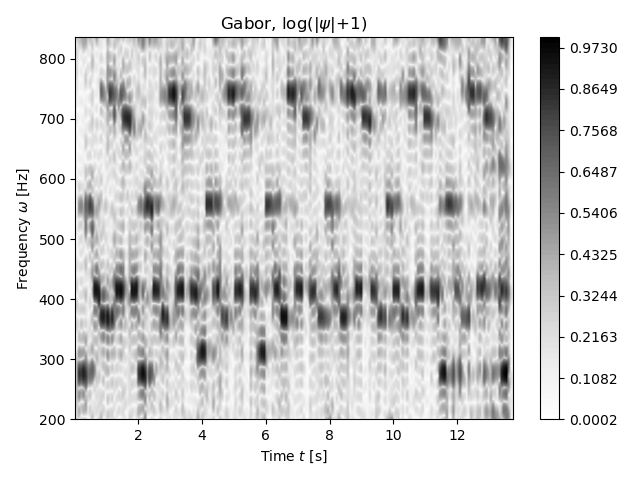
\includegraphics[width=0.45\textwidth]{gnr/gnr_gab_1000pt_window}\includegraphics[width=0.47\textwidth]{gnr/combined}
  \caption{Spectrogram of the first fourteen seconds of Guns and Roses' ``Sweet Child of Mine,'' computed by Gabor (left) and Gabor-Wigner (right) methods with $0.02$ s long Gabor window. The Gabor-Wigner approach resolves spectral lines better (predicting more localization in frequency) and hints at additional structure (chords) in the music through spectral lines at harmonic modulation (mean) frequencies. The original low D note (chord root) is carried up to G by the end of the intro section and repeats at 12 seconds.}\label{gnr}
\end{figure}

\begin{figure}[h!]
  \centering
  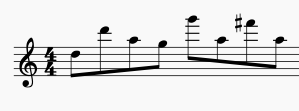
\includegraphics[width=0.45\textwidth]{music_score/gnr}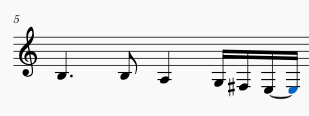
\includegraphics[width=0.44\textwidth]{music_score/floyd_option2}
  \caption{Identified scores for Sweet Child of Mine guitar riff (left) and Pink Floyd bass line (also 4-4, right) made in the free software ``MuseScore 3''. The bass line appears to repeat B before descending.}\label{score}
\end{figure}

\subsection{Comfortably Numb guitar solo bass line}
In a similar manner the bass line under the extremely sick Pink Floyd guitar solo was identified in Fig. \ref{floyd} through Gabor and Gabor-Wigner spectrograms, consisting of the notes B (124 Hz), A (110 Hz), G (98 Hz), F\# (90 Hz), and E (80 Hz) as detailed Fig. \ref{score}.

\begin{figure}[t!]
  \centering
  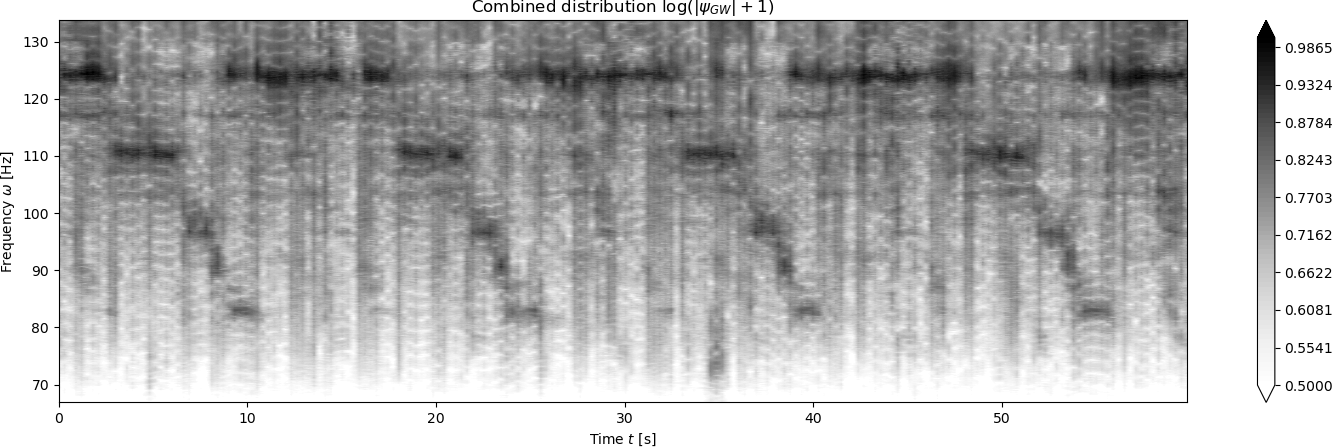
\includegraphics[width=0.9\textwidth]{floyd/floyd_gab_wig}
  \caption{Spectrogram of the bass line during the guitar solo in Pink Floyd's ``Comfortably Numb,'' computed by Gabor-Wigner transform with $0.023$ s long Gabor window. The bass line maintains a slow tempo throughout the mind-melting guitar solo and appears to consist of (on its long timescale) a dotted quarter and eighth (B), quarter note (A) , and descending three eighth notes (G, F\#, E).}\label{floyd}
\end{figure}

\subsection{Attempt at guitar solo in Comfortably Numb}
An attempt was made at part of the guitar solo in Pink Floyd. The Wigner filter was not used as it was too computationally expensive to extend so high into frequency for such a long clip on an $\mathcal{O}(N^2)$ operation, so the Gabor transform with FFT was used. The first five seconds of the Floyd guitar solo are examined in Fig. \ref{floyd_5s}. A lot of distortion is present which made the spectral signatures rather diffuse. A general structure is seen as a descending sequence of notes beginning on the first string, apparently in key of D.

\begin{figure}[b!]
  \centering
  \includegraphics[width=0.6\textwidth]{floyd_5s}
  \caption{Spectrogram of the first five seconds of the guitar solo in Pink Floyd's ``Comfortably Numb,'' computed by Gabor transform with $0.1$ s long Gabor window. Identified notes are circled and labelled.}\label{floyd_5s}
\end{figure}

% \begin{table}[b]
%   \centering
%   \begin{tabular}{|l|l|l|l|l|l|l|l|l|}
%     \hline
%     Time {[}hr{]}   & 0-3.5 & 3.5-7.0 & 7.0-10.5 & 10.5-14.0 & 14.0-17.5 & 17.5-21.0 & 21.0-24.5 & All-time average \\ \hline
%     $\langle k_x\rangle_T$ {[}1/L{]} & 0.814 & 0.661   & 0.784    & 0.760     & 0.810     & 0.728     & 0.802     & 0.766            \\ \hline
%     $\langle k_y\rangle_T$ {[}1/L{]} & 0.271 & 0.292   & 0.331    & 0.240     & 0.341     & 0.267     & 0.271     & 0.288            \\ \hline
%     $\langle k_z\rangle_T$ {[}1/L{]} & -1.00 & -1.03   & -1.09    & -1.06     & -1.13     & -1.07     & -1.1125   & -1.07            \\ \hline
%   \end{tabular}
%   \caption{Observed center frequencies of data following spectral averaging over time intervals of $3.5$ hours, with seven samples per interval, then used as the filter frequencies $k_0$ in the Gaussian filter. The arbitrary spatial unit is given as $L$, not to be confused with domain length. The all-time average is given as well.}\label{frequencies}
% \end{table}

% Note that in Table \ref{frequencies} negative wavenumbers are used as the given spatial data is complex, meaning that the reality condition is not satisfied, instead $\hat{f}(-k) = \hat{f}^*(k)$ in this dataset. The absolute value is reported as ``the frequency'' of the submarine, however. This identifies the submarine's spectral signature as $\bm{k} \approx \{0.766 \pm 0.05, 0.288 \pm 0.03, 1.07 \pm 0.04 \}$ {[}1/L{]} by mean and standard deviation of the window averages of Table \ref{frequencies}, where L is an arbitrary space unit corresponding to that of the provided data, \textit{not} the domain length. The width of the space or frequency ``submarine Gaussian'' was not measured for ease of analysis.

% Having computed the center frequencies, the spectrum was filtered and the trajectory determined according to the schematic Steps 4 and 5. The resulting 3D trajectory and top-down position given in Figs. \ref{traj:3d}, \ref{traj:2d} respectively. This suggests the submarine is currently located around $\bm{x}\sim(-5, 6.5)$ in $(x,y)$.

% \begin{figure}[hb]
%   \centering
%   \begin{subfigure}{0.42\textwidth}
%     \centering
%     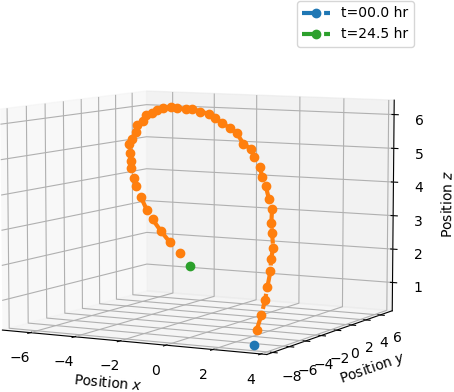
\includegraphics[width=0.99\linewidth]{pics/3d_traj}
%     \caption{Three-dimensional trajectory of submarine, showing a rise and dive maneuver.}\label{traj:3d}
%   \end{subfigure}
%   \begin{subfigure}{0.42\textwidth}
%     \centering
%     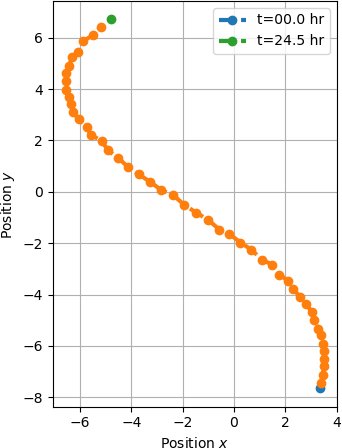
\includegraphics[width=0.6\linewidth]{pics/2d_traj}
%     \caption{Top-down view of predicted trajectory. Ideal search area for submarine-tracking aircraft is around $\bm{x} \sim (-5, 6.5)$ and continuing north-east.}\label{traj:2d}
%   \end{subfigure}
%   \caption{Identified submarine trajectory sampled 49 times in a 24.5 hour period, in 3D and 2D projections.}
% \end{figure}

% Summary and Conclusions
\section{Summary and Conclusions}
This numerical experiment combined the short-time Fourier transform (Gabor) with the Wigner distribution to enhance each other's spectral signatures. The combination of the two can be thought of as a filtered version of either, compromising between the strengths of each method. By this method the musical score was identified of two classic music clips. Python was used for implementations in this exercise.

% References
\bibliographystyle{unsrt}
\bibliography{references}

% Appendices
\begin{appendices}

  \newpage
  \section{Wigner distributions of periodic functions}\label{periodic}
  A remarkable property of the Wigner distribution is that it is straightforward (though computationally expensive) to calculate once a Fourier analysis of the function $f(t)$ has been determined. To see this, consider a periodic function expressed by its Fourier series,
\begin{equation}
  f(t) = \sum_{n=-\infty}^\infty c_ne^{i\omega_nt},\quad\quad \omega_n = \frac{2\pi}{L}n
\end{equation}
where $f(t+L)=f(t)$. Note that the function $f(t)$ is continuous in $t$ but discrete in its spectrum. The Wigner function inherits this property. Substituting into Eqn. \ref{wig}, one has
\begin{equation}
  W(t,\omega) = \sum_{n=-\infty}^\infty\sum_{m=-\infty}^\infty (c_ne^{i\omega_n t})^*(c_me^{i\omega_m t})\frac{1}{2\pi}\int_{-\infty}^\infty e^{-i(\omega-(\omega_n+\omega_m)/2)\tau}d\tau
\end{equation}
which then simplifies from the orthogonality of the Fourier basis into the expression
\begin{equation}
  W(t,\omega) = \sum_{n=-\infty}^\infty\sum_{m=-\infty}^\infty (c_ne^{i\omega_nt})^*(c_me^{i\omega_mt})\delta\Big(\omega - \frac{1}{2}(\omega_n+\omega_m)\Big).
\end{equation}
The summation is on the infinite lattice $(n,m)\in\mathbb{Z}^2$, yet the delta function restricts the frequency spectrum to be discrete. The comb picks out all frequencies $\omega$ integer multiples of \textit{half} the fundamental frequency,
\begin{equation}
  \omega = \frac{\pi}{L}\ell,\quad \ell\in\mathbb{Z}.
\end{equation}
From the frequency-matching condition and summation on diagonals of the lattice one has
\begin{equation}
  W\Big(t,\frac{\pi}{L}\ell\Big) = \sum_{n=-\infty}^\infty(c_ne^{i\omega_nt})^*(c_{\ell-n}e^{i\omega_{\ell - n}t}),\quad \ell\in\mathbb{Z}
\end{equation}
as shown in Fig. \ref{lattice}. Note that if the function $f(t)$ is real, then the Wigner distribution $W(t,\omega)$ is also real. This calculation reveals the Wigner function as particularly simple in the Fourier basis, being just a discrete convolution of the Fourier series with itself for each $\ell$. For example, the zero-mode is the summation
\begin{equation}
  W(t, 0) = \sum_{n=-\infty}^\infty|c_n|^2e^{-i2\omega_nt}
\end{equation}
which has zero time-average (contributing nothing to the spectrum $\hat{f}(\omega)$) but necessary to describe the \textit{local} (in coordinate $t$) deviation from mean-zero in a function's spatial energy distribution. As an energy it oscillates with twice the frequency of its corresponding mode. In order to avoid aliasing interference the distribution should be truncated at the Nyquist frequency of the series,
\begin{equation}
  W\Big(t, \frac{\pi}{L}\ell\Big) = \sum_{n=-k}^k(c_ne^{i\omega_nt})^*(c_{\ell-n}e^{i\omega_{\ell - n}t}),\quad \ell\in\mathbb{Z}.\label{full_wig}
\end{equation}

\begin{figure}[b!]
  \centering
  \includegraphics[width=0.28\textwidth]{lattice_sum}
  \caption{Summation on the lattice $(n,m)$ resolves into a single summation on a diagonal satisfying $m=\ell-n$ for each frequency component $\ell$ of the Wigner distribution.}\label{lattice}
\end{figure}

\subsection{Wigner distribution of an analytic signal}\label{analytic}
The \textit{analytic signal} $f_s(t)$ joins the Hilbert transform of a function $f(t)$ to itself,
\begin{equation}
  f_s(t) = f(t) + i\mathcal{H}[f](t).
\end{equation}
If a signal is real-valued then the spectrum of its analytic signal is the one-sided series
\begin{equation}
  f_s(t) = \sum_{n=0}^\infty 2c_ne^{i\omega_nt},\quad \omega_n = \frac{2\pi}{L}.
\end{equation}
In signal processing this is called the ``real Fourier series''. If desired, one can eliminate the interference effects at the low-frequencies present in the Wigner distribution of Eqn. \ref{full_wig}. It should be noted that this process will discard the beat effects, and the marginal distribution will be altered to instead return the intensity spectrum of the analytic signal $|f_s(t)|^2$. This can be useful in data analysis however, and the formula for the Wigner distribution simplifies.

Repeating the calculation of Section \ref{periodic}, the distribution of $f_s(t)$ is given by \cite{wigner_periodic}
\begin{equation}
  W\Big(t, \frac{\pi}{L}\ell\Big) = 2\sum_{n=0}^\infty\sum_{m=0}^\infty (c_ne^{i\omega_nt})^*(c_me^{i\omega_mt})\delta\Big(\frac{\pi}{L}(\ell - (n+m))\Big),\quad \ell\in\mathbb{Z}^+.
\end{equation}
The summation is now in the first quadrant only of the lattice in Fig. \ref{lattice}, and the summation along the diagonal $m = \ell - n$ truncates. For a given mode $\ell$, interference is possible only between frequencies up to and including $\ell$, giving
\begin{equation}
  W\Big(t, \frac{\pi}{L}\ell\Big) = 2\sum_{n=0}^\ell(c_ne^{i\omega_nt})^*(c_{\ell-n}e^{i\omega_{\ell-n}t}),\quad \ell\in\mathbb{Z}^+.
\end{equation}
This reduces interferences but discards important information regarding \textit{frequency differences}, instead describing only frequency-sum modulations. For example, beat frequencies $f_b = |f_2-f_1|$ are described by the Wigner distribution of an analytic signal more like the corresponding Gabor transform.

% \subsection{Transform of the covariance function}
% If instead one considers the Fourier transform of the instantaneous \textit{correlation} or covariance of two functions $x(t)$ and $y(t)$, a cross-term Wigner function can be defined
% \begin{equation}
%   W_{\{x,y\}}(t, \omega) = \int_{-\infty}^\infty x^*\Big(t-\frac{\tau}{2}\Big)y\Big(t+\frac{\tau}{2}\Big)e^{-i\omega\tau}d\tau.
% \end{equation}
% If $x(t)$ and $y(t)$ have the same period, then $W_{\{x,y\}}$ is the convolution of the two Fourier series,
% \begin{align}
%   x(t) = \sum_{n=-\infty}^\infty a_ne^{i\omega_nt},&\quad\quad y(t) = \sum_{n=-\infty}^\infty b_ne^{i\omega_nt}\\
%   W_{\{x,y\}}(t,\frac{\pi}{L}\ell) &= \sum_{n=-\infty}^\infty (a_ne^{i\omega_nt})^*(b_{\ell-n}e^{i\omega_{\ell-n}t}).
% \end{align}
% Its marginals are the correlation function in frequency and function $x(t)\times y(t)$ in space.


\newpage
\section{Examples of Wigner distributions}\label{examples}
The following are simple examples of Wigner functions presented in order to build intuition. An objective of the following discussion is to point out that the interference patterns present in the distribution are physically meaningful, but are perhaps undesirable from a signal processing perspective, in particular if the signal is not truly periodic (e.g. a music recording).

\subsection{Single sine function}
The distribution of a basic sine function $f(t) = \sin(t) = -\frac{1}{2}ie^{it} + \frac{1}{2}ie^{-it}$ is given by
\begin{equation}
  W\Big(t,\frac{\pi}{L}\ell\Big) = \frac{1}{4}\begin{cases} 1& \ell = 2\\
    -2\cos(2t) & \ell = 0\\
    1 & \ell = -2
  \end{cases}
\end{equation}
so that summing in $\ell$, one finds the energy distribution $|f(t)|^2 = \frac{1}{2}-\frac{1}{2}\cos(2t) = \sin^2(t)$. The Wigner distribution is shown below in Fig. \ref{sine_fig}. Evidently the interference pattern at $\ell=0$ is due to combination of the positive and negative frequency components. In the signal processing context it is remarked that the zero-mode is ``unexpected'', but this example demonstrates that it is necessary in order to describe the non-zero mean in energy of the sine wave. The zero-mode $\frac{1}{2}\cos(2t)=0$ when $f(t) = |f(t)|^2$ and no more energy is needed than that present in $\ell=\pm 2$.
\begin{figure}[ht!]
  \centering
  \includegraphics[width=0.435\textwidth]{sine/sine}
  \includegraphics[width=0.45\textwidth]{sine/sine_wig}
  \caption{Wigner function of the sine wave (right), note interference between modes $n=\pm 1$.}\label{sine_fig}
\end{figure}

\subsection{Classic beat wave}
Now consider a function with more spatially modulated structure than the sine wave,
\begin{equation}
  f(t) = \cos(4t) + \cos(5t) = 2\cos\Big(\frac{1}{2}t\Big)\cos\Big(\frac{9}{2}t\Big).
\end{equation}
This waveform has a classic beat structure as shown in Fig. \ref{beat_fig}, with a low-frequency of $\omega_B = 1/2$  and a modulation frequency of $\omega_M = 9/2$. The spectrum of the signal (its orthogonal components) is of course only present at $\omega = 4$ and $5$, but the spatial structure of the waveform has a \textit{low-frequency variation} which is present in the mode $\omega = 0.5$ and a \textit{harmonic modulation frequency} at $\omega = 4.5$. A generic spectrogram computed by a windowed Fourier transform will typically not see the energy present in the harmonic combinations resulting in spatial structure of the waveform (appearing instead as a bump).

\begin{figure}[ht!]
  \centering
  \includegraphics[width=0.435\textwidth]{wigner_tests/classic_beat/classic_beat}
  \includegraphics[width=0.45\textwidth]{wigner_tests/classic_beat/wigner}
  \caption{Spatial modulation in the superposition of $\cos(4t)$ and $\cos(5t)$ (left) and Wigner distribution (right). Low-frequency energy is present in modes $\ell = 0, \pm 1$ and high-frequency modulation in $\omega = 9/2$ which cancel out when considering the total frequency spectrum.}\label{beat_fig}
\end{figure}

\subsection{Elliptic cosine}
Another good example of spatial structure is the elliptic cosine function with Fourier series
\begin{equation}
  \text{cn}(4K(m)x|m) = \frac{\pi}{K(m)\sqrt{m}}\sum_{n=0}^\infty\frac{\cos(2\pi(1+2n)x)}{\cosh(\frac{\pi}{2}(1+2n)\frac{K'(m)}{K(m)})}.
\end{equation}
where $K(m)$ is a complete elliptic integral. For parameter $m$ close to one the wave energy becomes very localized, shown in Fig. \ref{ell_cos}. Where the function is peaked there is a zero-mode (DC) component to the energy! However in its totality there is no mean value to the function. In order to cancel out this zero-mode a \textit{virtual frequency distribution} is present in coordinate $x$ where the signal energy is entirely zero. This phenomenon can be understood as a ``spatial beat'' in constrast to the usual frequency beat. In the context of the energetic distribution of a truly periodic signal this interference phenomenon has physical significance. 

\begin{figure}[b!]
  \centering
  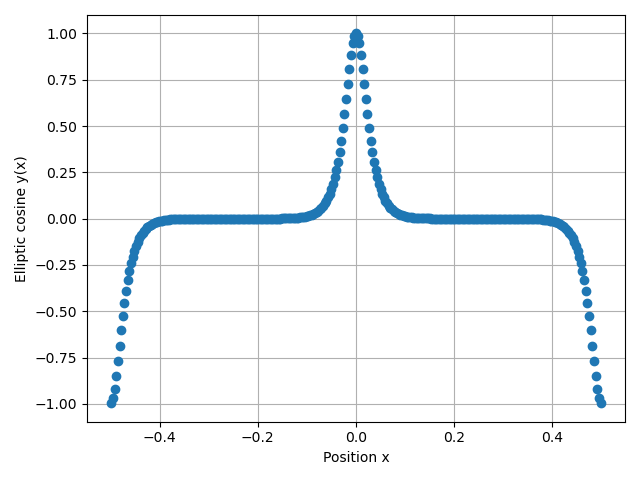
\includegraphics[width=0.435\textwidth]{wigner_tests/elliptic_cosine/elliptic_cosine}
  \includegraphics[width=0.45\textwidth]{wigner_tests/elliptic_cosine/wigner_elcos}
  \caption{Elliptic cosine and its Wigner distribution for parameter $m=1 - 1^{-10}$.}\label{ell_cos}
\end{figure}

\subsection{D Major arpeggio on the guitar}
Yet for analysis of a waveform \textit{assumed} to be periodic the spatial beat effect is detrimental. An example of such is in analysis of a musical waveform. Below the Wigner function (of the analytic signal, c.f. Section \ref{analytic}) is calculated of the four notes of a D Major chord played in succession. The four notes of the D chord are 144 Hz (D), 216 Hz (A), 288 Hz (D), and 364 Hz (F\#). A windowed Fourier transform is also computed and shown for comparison, which has only four spectral lines (plus their integer harmonics).

\begin{figure}[t!]
  \centering
  \includegraphics[width=0.45\textwidth]{music_experiments/DArp/wigner}
  \includegraphics[width=0.45\textwidth]{music_experiments/DArp/gabor}
  \caption{Wigner distribution (left) and typical spectrogram (right) of four notes played on the guitar, each calculated from the analytic signal of the waveform. The Wigner function has an interference pattern where the signal is silent (0-1.1 s and the end). It also describes interferences between each pair of notes, in particular at the chord center frequency of $254$ Hz, (with a role in the chord's psychoacoustical perception).}\label{wig_gabor}
\end{figure}

The Wigner function results in more localized signals, but also encounters \textit{time beats} when the recording is silent (a purely artificial effect). It also predicts \textit{interferences} between any pair of notes. One of the pleasant aspects of the D Major chord is its internal harmony, as shown in Table \ref{DChord}. The frequency of modulation between any pair of notes reinforce one another and fill out the succeeding intervals. The Wigner spectrogram picks up this interference pattern and indicates frequencies and relationships which may be \textit{perceived} but not present in the orthogonal decomposition. A compromise distribution is shown in Fig. \ref{wig_gabor}.

\begin{table}[h]
  \centering
\begin{tabular}{|l|l|l|l|l|l|l|l|}
\hline
Chord Notes {[}Hz{]}          & F\#, 364 &     & D, 288 &     & A, 216 &     & D, 144 \\ \hline
First Neighbor Mean {[}Hz{]}  &           & 326 &         & 252 &         & 180 &         \\ \hline
Second Neighbor Mean {[}Hz{]} &           &     & 290     &     & 216     &     &         \\ \hline
Center Frequency {[}Hz{]}     &           &     &         & 254 &         &     &         \\ \hline
\end{tabular}
\caption{Frequencies of modulation in the D Major chord on the guitar.}\label{DChord}
\end{table}

\begin{figure}[hb!]
  \centering
  \includegraphics[width=0.46\textwidth]{music_experiments/DArp/combined}
  \caption{The combined spectrogram multiplies the windowed Fourier transform with the Wigner distribution. The resulting spectrogram separates the true signal from its ``time beat'' phantom part and includes spectral lines at the frequencies of modulation between the component notes of the arpeggiated D chord.}\label{wig_gabor}
\end{figure}

\newpage
% MATLAB Functions
\section{Python Functions}\label{functions}
The following list compiles important Python functions used in implementation:
\begin{itemize}
\item \texttt{soundfile.read} is used to read in a \texttt{.wav} file as a list along with sample rate
\item \texttt{numpy.fft.rfft} computes only the positive frequency components of the Fourier transform, used to construct the analytic signal of the time series.
\item \texttt{numba.cuda.jit} is used to GPU-accelerate the brute-force calculation of the Wigner function.
\item \texttt{numpy.roll} is used to roll the Gabor window of a specified number of points across the time series domain.
\end{itemize}

% MATLAB Codes
\section{Python Implementation}\label{implementation}
Wigner function file \texttt{fourier.py}:
\lstinputlisting{fourier.py}
\vspace{5cm}
Main implementation file \texttt{hw2.py}:
\lstinputlisting{hw2.py}
% \begin{listing}[h]
% \inputminted{matlab}{example.m}
% \caption{Example code from external file.}
% \label{listing:examplecode}
% \end{listing}

\end{appendices}

\end{document}